\documentclass[12pt]{article}
\usepackage{afterpage}
\usepackage{amsmath}
\usepackage{amsfonts}
\usepackage{amssymb}
\usepackage{amsbsy}
\usepackage{bm}
\usepackage{epsfig}
\usepackage{rotating}
\usepackage{setspace}
\usepackage{tabls}
\usepackage{hhline}
\usepackage{float}
\usepackage{subfigure}
\usepackage{float}
\usepackage{xspace}
%\usepackage{subfigmat}
%\usepackage{citesort}
%\usepackage{cites}
%\usepackage{overcite}
%\usepackage[section]{placeins}

% uncomment for submission of manuscript to NSE
\usepackage[nolists, nomarkers]{endfloat}
%
% use to include postscript figures
\usepackage{graphicx,color}
%
%\usepackage[light,firsttwo]{draftcopy}
%\draftcopySetGrey{0.90}

%\usepackage{dbl}

% -----------------------------------------------------------------------------
% define newcommands
% -----------------------------------------------------------------------------

%\setlength{\floatsep}{4pt plus 1pt minus 1pt}
%\setlength{\textfloatsep}{8pt plus 1pt minus 1pt}
%\setlength{\intextsep}{4pt plus 1pt minus 1pt}
%\setlength{\abovedisplayskip}{4pt plus 1pt minus 1pt}
%\setlength{\belowdisplayskip}{4pt plus 1pt minus 1pt}

\makeatletter
\renewcommand{\@thesubfigure}{\thefigure\thesubfigure\space}
\makeatother
% =================================================================================================
% more new commands
% +++++++++++++++++++++++++++++++++++++++++++++++++++++++++++++++++++++++++++++++++++++++++++++++++
\setlength{\textwidth}{6.5in}
\setlength{\textheight}{8.in}
\setlength{\oddsidemargin}{0in}
%\setlength{\topmargin}{0.75in}
\setlength{\headsep}{12pt}
%\addtolength{\oddsidemargin}{-0.5in}
%\addtolength{\textwidth}{1.0in}
%\addtolength{\textheight}{1.0in}
\renewcommand{\thefootnote}{\fnsymbol{footnote}}
%
% -----------------------------------------------------------------------------
% define newcommands
% -----------------------------------------------------------------------------

%\setlength{\floatsep}{4pt plus 1pt minus 1pt}
%\setlength{\textfloatsep}{8pt plus 1pt minus 1pt}
%\setlength{\intextsep}{4pt plus 1pt minus 1pt}
%\setlength{\abovedisplayskip}{4pt plus 1pt minus 1pt}
%\setlength{\belowdisplayskip}{4pt plus 1pt minus 1pt}

% =================================================================================================
% more new commands
% +++++++++++++++++++++++++++++++++++++++++++++++++++++++++++++++++++++++++++++++++++++++++++++++++

% Ways of grouping things
%
\newcommand{\bracket}[1]{\left[ #1 \right]}
\newcommand{\bracet}[1]{\left\{ #1 \right\}}
\newcommand{\fn}[1]{\left( #1 \right)}
\newcommand{\ave}[1]{\left\langle #1 \right\rangle}
%
% Derivative forms
%
\newcommand{\dx}[1]{\,d#1}
\newcommand{\dxdy}[2]{\frac{\partial #1}{\partial #2}}
\newcommand{\dxdt}[1]{\frac{\partial #1}{\partial t}}
\newcommand{\dxdz}[1]{\frac{\partial #1}{\partial z}}
\newcommand{\dddx}[1]{\frac{d #1}{d x}}
\newcommand{\dfdt}[1]{\frac{\partial}{\partial t} \fn{#1}}
\newcommand{\dfdz}[1]{\frac{\partial}{\partial z} \fn{#1}}
\newcommand{\ddt}[1]{\frac{\partial}{\partial t} #1}
\newcommand{\ddz}[1]{\frac{\partial}{\partial z} #1}
\newcommand{\dd}[2]{\frac{\partial}{\partial #1} #2}
\newcommand{\ddx}[1]{\frac{\partial}{\partial x} #1}
\newcommand{\ddy}[1]{\frac{\partial}{\partial y} #1}
%
% Vector forms
%
%\renewcommand{\vec}[1]{\ensuremath{\stackrel{\rightarrow}{#1}}}
%\renewcommand{\div}{\ensuremath{\vec{\nabla} \cdot}}
%\newcommand{\grad}{\ensuremath{\vec{\nabla}}}
\renewcommand{\vec}[1]{\overrightarrow{#1}}
\renewcommand{\div}{\vec{\nabla}\! \cdot \!}
\newcommand{\grad}{\vec{\nabla}}
\newcommand{\oa}[1]{\fn{\frac{1}{3}\hat{\Omega}\!\cdot\!\overrightarrow{A_{#1}}}}

%
% Equation beginnings and endings
%
\newcommand{\bea}{\begin{eqnarray}}
\newcommand{\eea}{\end{eqnarray}}
\newcommand{\be}{\begin{equation}}
\newcommand{\ee}{\end{equation}}
\newcommand{\beas}{\begin{eqnarray*}}
\newcommand{\eeas}{\end{eqnarray*}}
\newcommand{\bdm}{\begin{displaymath}}
\newcommand{\edm}{\end{displaymath}}


%
% Equation punctuation
%
\newcommand{\pec}{\; ,}
\newcommand{\pep}{\; .}
%
% Equation labels and references, figure references, table references
%
\newcommand{\LEQ}[1]{\label{eq:#1}}
\newcommand{\EQ}[1]{Eq.~(\ref{eq:#1})}
\newcommand{\EQS}[1]{Eqs.~(\ref{eq:#1})}
\newcommand{\REQ}[1]{\ref{eq:#1}}
\newcommand{\LFI}[1]{\label{fi:#1}}
\newcommand{\FI}[1]{Fig.~\ref{fi:#1}}
\newcommand{\RFI}[1]{\ref{fi:#1}}
\newcommand{\LTA}[1]{\label{ta:#1}}
\newcommand{\TA}[1]{Table~\ref{ta:#1}}
\newcommand{\RTA}[1]{\ref{ta:#1}}

%
% List beginnings and endings
%
\newcommand{\bl}{\bss\begin{itemize}}
\newcommand{\el}{\vspace{-.5\baselineskip}\end{itemize}\ess}
\newcommand{\ben}{\bss\begin{enumerate}}
\newcommand{\een}{\vspace{-.5\baselineskip}\end{enumerate}\ess}
%
% Figure and table beginnings and endings
%
\newcommand{\bfg}{\begin{figure}}
\newcommand{\efg}{\end{figure}}
\newcommand{\bt}{\begin{table}}
\newcommand{\et}{\end{table}}
%
% Tabular and center beginnings and endings
%
\newcommand{\bc}{\begin{center}}
\newcommand{\ec}{\end{center}}
\newcommand{\btb}{\begin{center}\begin{tabular}}
\newcommand{\etb}{\end{tabular}\end{center}}
%
% Single space command
%
%\newcommand{\bss}{\begin{singlespace}}
%\newcommand{\ess}{\end{singlespace}}
\newcommand{\bss}{\singlespacing}
\newcommand{\ess}{\doublespacing}
%
%---New environment "arbspace". (modeled after singlespace environment
%                                in Doublespace.sty)
%   The baselinestretch only takes effect at a size change, so do one.
%
\def\arbspace#1{\def\baselinestretch{#1}\@normalsize}
\def\endarbspace{}
\newcommand{\bas}{\begin{arbspace}}
\newcommand{\eas}{\end{arbspace}}
%
% An explanation for a function
%
\newcommand{\explain}[1]{\mbox{\hspace{2em} #1}}
%
% Quick commands for symbols
%
\newcommand{\half}{\frac{1}{2}}
\newcommand{\halff}{1/2}
\newcommand{\third}{\frac{1}{3}}
\newcommand{\twothird}{\frac{2}{3}}
\newcommand{\mdot}{\dot{m}}
\newcommand{\ten}[1]{\times 10^{#1}\,}
\newcommand{\cL}{{\cal L}}
\newcommand{\cD}{{\cal D}}
\newcommand{\cF}{{\cal F}}
\newcommand{\cE}{{\cal E}}
\renewcommand{\Re}{\mbox{Re}}
\newcommand{\Ma}{\mbox{Ma}}
%
% Inclusion of Graphics Data
%
%\input{psfig}
%\psfiginit
%
% More Quick Commands
%
\newcommand{\bi}{\begin{itemize}}
\newcommand{\ei}{\end{itemize}}
\newcommand{\dxi}{\Delta x_i}
\newcommand{\dyj}{\Delta y_j}
\newcommand{\ts}[1]{\textstyle #1}
% Mark URL's
\newcommand{\URL}[1]{{\textcolor{blue}{#1}}}



% Alter some LaTeX defaults for better treatment of figures:
    % See p.105 of "TeX Unbound" for suggested values.
    % See pp. 199-200 of Lamport's "LaTeX" book for details.
    %   General parameters, for ALL pages:
    \renewcommand{\topfraction}{0.9}	% max fraction of floats at top
    \renewcommand{\bottomfraction}{0.8}	% max fraction of floats at bottom
    %   Parameters for TEXT pages (not float pages):
    \setcounter{topnumber}{2}
    \setcounter{bottomnumber}{2}
    \setcounter{totalnumber}{2}     % 2 may work better
    \setcounter{dbltopnumber}{2}    % for 2-column pages
    \renewcommand{\dbltopfraction}{0.9}	% fit big float above 2-col. text
    \renewcommand{\textfraction}{0.07}	% allow minimal text w. figs
    %   Parameters for FLOAT pages (not text pages):
    \renewcommand{\floatpagefraction}{0.7}	% require fuller float pages
	% N.B.: floatpagefraction MUST be less than topfraction !!
    \renewcommand{\dblfloatpagefraction}{0.7}	% require fuller float pages

	% remember to use [htp] or [htpb] for placement

\newcommand{\SN}{S$_N$\xspace}
\renewcommand{\vec}[1]{\bm{#1}} %vector is bold italic
\newcommand{\vd}{\bm{\cdot}} % slightly bold vector dot
\newcommand{\ud}{\mathop{}\!\mathrm{d}} % upright derivative symbol
\newcommand{\pderiv}[2]{\frac{\partial #1}{\partial #2}}
\newcommand{\dderiv}[2]{\frac{\ud #1}{\ud #2}}
\newcommand{\edd}{\langle \mu^2 \rangle} 
	
	
% =================================================================================================
\date{}

\begin{document}

%\bibliographystyle{nse}
%\bibnum{p}

\thispagestyle{empty}
\bc
{\Large \bf Variable Eddington Factor for Mixed Hybrid Finite Element/Linear Discontinuous Galerkin Source Iteration}\\
\vspace{0.5in}
{\large {\bf S. Olivier, J.E. Morel}\\
$ $\\
Department of Nuclear Engineering\\
Texas A\&M University\\
College Station, TX 77843}\\
\ec
$ $\\
\bc
{\large \bf Abstract}\\
\ec
\noindent
\emph{
Abstract goes here
}\\
$ $\\
\noindent
{\bf Keywords}\\
\noindent P$_N$ equations, S$_N$ equations, asymptotic decay lengths.\\
$ $\\
\noindent {\bf Running Head}\\
\noindent Asymptotic S$_{N+1}$ Equations\\
$ $\\
\noindent{\bf Corresponding Author}\\
\noindent Jim E. Morel, Phone: (979)845-6072, FAX: (979)845-6075, E-mail: \emph{morel@tamu.edu}.
$ $\\
\newpage
\ess

\section{Introduction}

\section{Variable Eddington Method}
%!TEX root = ./jctt.tex

\subsection{Source Iteration}
The steady-state, mono-energetic, isotropically-scattering, fixed-source Linear Boltzmann Equation in slab geometry is: 
	\begin{equation} \label{eq:bte}
		\mu \pderiv{\psi}{x}(x, \mu) + \Sigma_t(x) \psi(x,\mu) = 
		\frac{\Sigma_s(x)}{2} \int_{-1}^{1} \psi(x, \mu') d\mu' + \frac{Q(x)}{2} \,,
	\end{equation}
where $\mu = \cos\theta$ is the cosine of the angle of flight $\theta$ relative to the $x$--axis, $\Sigma_t(x)$ and $\Sigma_s(x)$ the total and scattering macroscopic cross sections, $Q(x)$ the isotropic fixed-source and $\psi(x, \mu)$ the angular flux \cite{adams}. Applying the Discrete Ordinates (\SN) angular discretization yields the following system of $N$ coupled, ordinary differential equations: 
	\begin{equation} \label{eq:sn}
		\mu_n \dderiv{\psi_n}{x}(x) + \Sigma_t(x) \psi_n(x) = 
		\frac{\Sigma_s(x)}{2} \phi(x) + \frac{Q(x)}{2} \,, 1 \leq n \leq N \,,
	\end{equation}
where $\psi_n(x) = \psi(x, \mu_n)$ is the discrete angular flux. The scalar flux is computed using an $N$-point quadrature rule where the quadrature weights, $w_n$, sum to two. In other words, 
	\begin{equation} 
		\phi(x) = \sum_{n=1}^N w_n \psi_n(x)
	\end{equation}
The Source Iteration (SI) scheme lags the flux in the scattering term resulting in a system of $N$ independent, first-order, ordinary differential equations: 
	\begin{equation} \label{eq:si}
			\mu_n \dderiv{\psi_n^{\ell+1}}{x}(x) + \Sigma_t(x) \psi_n^{\ell+1}(x) = 
			\frac{\Sigma_s(x)}{2} \phi^{\ell}(x) + \frac{Q(x)}{2} \,, 1 \leq n \leq N \,,
		\end{equation}
where the superscripts indicate the iteration index. 

\subsection{Variable Eddington Factor Acceleration}
The Eddington equations are found by taking the first two angular moments of Eq. \ref{eq:bte}: 
	\begin{subequations} 
	\begin{equation} \label{eq:zero}
		\dderiv{}{x} J(x) + \Sigma_a(x) \phi(x) = Q(x) \,,
	\end{equation} 
	\begin{equation} \label{eq:first}
		\frac{\ud}{\ud x} \edd(x) \phi(x) + \Sigma_t(x) J(x) = 0 \,,
	\end{equation}
	\end{subequations}
where $\phi(x) = \int_{-1}^1 \psi(x,\mu) \ud \mu$ is the scalar flux, $J(x) = \int_{-1}^{1} \mu \psi(x, \mu) \ud \mu$ the current and 
	\begin{equation} \label{eq:eddington} 
		\edd(x) = \frac{\int_{-1}^1 \mu^2 \psi(x, \mu) \ud \mu}{\int_{-1}^1 \psi(x, \mu) \ud \mu}
		% \xrightarrow{\text{S}_N} \frac{\sum_{n=1}^N \mu_n^2 w_n\psi_n(x)}{\sum_{n=1}^N w_n \psi_n(x)} 
	\end{equation}
the Eddington factor. 

This formulation is beneficial because Eq. \ref{eq:zero} is a conservative balance equation and---if $\edd(x)$ is known---the Eddington equations' system of two first-order, ordinary differential equations can be solved directly with well-established methods. However, computing $\edd(x)$ requires knowledge of the angular flux. 

In VEF, \SN is used to compute the Eddington factor needed to solve the Eddington equations. Source iteration is then:  
	\begin{enumerate}
		\item Given the previous estimate for the scalar flux, $\phi^{\ell}(x)$, solve Eq. \ref{eq:si} for $\psi_n^{\ell+1/2}(x)$. 
		\item Compute $\edd^{\ell+1/2}(x)$ with Eq. \ref{eq:edd_sn}. 
		% \item Interpolate $\edd(x)$ onto the MFEM grid 
		\item Solve the Eddington equations for $\phi^{\ell+1}(x)$ using $\edd^{\ell+1/2}(x)$. 
		% \item Use the Eddington equations' $\phi(x)$ on the right hand side of Eq. \ref{eq:si}.  
		\item Update the scalar flux estimate on the right side of Eq. \ref{eq:si} with $\phi^{\ell+1}(x)$ and repeat the iteration process until the scalar flux converges. 
	\end{enumerate}
% This process is one source iteration consisting of an \SN transport step to compute the Eddington factor and an MFEM acceleration step to compute $\phi(x)$. The scalar flux from the acceleration step is used in the right hand side of Eq. \ref{eq:si} and steps 1--4 are repeated until the acceleration step's $\phi(x)$ converges according to Eq. \ref{eq:converg}.  

Acceleration occurs because the angular shape of the angular flux, and thus the Eddington factor, converges much faster than the scalar flux. In addition, the Eddington equations model the contributions of all scattering events at once, reducing the dependence on source iterations to introduce scattering information. The solution from the Eddington equations is then an approximation for the full flux and not the $\ell - 1$ collided flux as it was without acceleration. 

In addition to acceleration, this scheme allows the \SN equations and Eddington equations to be solved with different spatial discretization methods. \SN can be spatially discretized using normal methods, such as Linear Discontinuous Galerkin, while the Eddington equations can be solved with MFEM. 

\subsection{Lumped Linear Discontinuous Galerkin \SN}
The LLDG discretization of Eq. \ref{eq:sn} is:
	\begin{subequations} \label{eq:lldg}
	\begin{equation} 
		\mu_n \left(\psi_{n,i} - \psi_{n, i-1/2}\right) + \frac{\Sigma_{t,i} h_i}{2} \psi_{n,i}^L
		= \frac{\Sigma_{s,i} h_i}{4} \phi_i^L + \frac{h_i}{4} Q_i^L \,, 1 \leq n \leq N \,, 1 \leq i \leq I\,, 
	\end{equation}
	\begin{equation}
		\mu_n \left(\psi_{n,i+1/2} - \psi_{n,i}\right) + \frac{\Sigma_{t,i} h_i}{2} \psi_{n,i}^R
		= \frac{\Sigma_{s,i} h_i}{4} \phi_i^R + \frac{h_i}{4} Q_i^R \,, 1 \leq n \leq N \,, 1 \leq i \leq I\,,
	\end{equation}
	\end{subequations}
where $h_i$, $\Sigma_{t,i}$, and $\Sigma_{s,i}$ are the cell width, total cross section, and scattering cross section in cell $i$. The cell-edged angular fluxes are found through upwinding: 
	\begin{subequations}
	\begin{equation}
		\psi_{n,i-1/2} = \begin{cases}
			\psi_{n,i-1}^R & \mu_n > 0 \\
			\psi_{n,i}^L & \mu_n < 0
		\end{cases}
	\end{equation}
	\begin{equation}
		\psi_{n,i+1/2} = \begin{cases}
			\psi_{n,i}^R & \mu_n > 0 \\
			\psi_{n,i+1}^L & \mu_n < 0
		\end{cases}
	\end{equation}
	\end{subequations}
and the cell-centered angular flux is computed with:
	\begin{equation} \label{eq:psicent}
		\psi_{n,i} = \half \left(\psi_{n,i}^L + \psi_{n,i}^R\right) \,. 
	\end{equation}

In \SN, the Eddington factor is 
	\begin{equation} \label{eq:edd_sn}
		\edd(x) = \frac{\sum_{n=1}^N \mu_n^2 w_n\psi_n(x)}{\sum_{n=1}^N w_n \psi_n(x)} \,.
	\end{equation}

\subsection{Mixed Finite Element Method Eddington}


\subsection{Data Reconstruction}
	Data reconstruction methods are required to recover the linear discontinuous representation in LDG from the piecewise constant with discontinuous jumps at the cell edges representation in MFEM. Data reconstruction methods use neighboring cell centers or edges to extrapolate the MFEM flux to determine the discontinuous cell edge values in LDG that maintain the average and slope. Two data reconstruction methods have been implemented: one that uses the slope between the MFEM edge values and one that only uses cell centered values. 

	The first method sets the LDG discontinuous left and right fluxes in cell $i$, $\phi_{i,L}$ and $\phi_{i,R}$ to 
		\begin{equation}
			\phi_{i,L/R} = \phi_i \mp \frac{1}{2} \left(\phi_{i+1/2} - \phi_{i-1/2}\right)
		\end{equation}

	The second method uses a van Leer slope limiter on the MFEM cell centers. 

\section{Computational Results}
%!TEX root = ./jctt.tex

The order of accuracy, diffusion limit, and solution convergence were tested in 1D slab geometry with two Eddington factor representations and two scattering term reconstruction methods. The Eddington factor was represented as a piecewise constant with discontinuous jumps at the cell edges and as linear function using the MFEM basis functions. The scattering term reconstruction methods were no reconstruction and maintaining van Leer limited slopes with the MFEM cell centers. The no reconstruction method set the the left and right discontinuous scalar flux to the MFEM edge scalar flux:
	\begin{equation} 
		\phi_{i,L/R} = \phi_{i\mp1/2} \,,
	\end{equation}
where the left hand side is the flux used in the LLDG scattering term and the right hand side the MFEM drift diffusion scalar flux. 
% Maintaining slopes with the MFEM edge values was done according to: 
% 	\begin{equation} \label{eq:edgeReconstruction}
% 		\phi_{i,L/R} = \phi_i \mp \half\left(\phi_{i+1/2} - \phi_{i-1/2}\right) \,.
% 	\end{equation}
The van Leer cell centered reconstruction is: 
	\begin{equation} \label{eq:vanLeer}
		\phi_{i,L/R} = \phi_i \mp \frac{1}{4} \xi_\text{van Leer} \left[ \left(\phi_{i+1} - \phi_{i}\right) + 
			\left(\phi_{i} - \phi_{i-1}\right)\right] \,
	\end{equation}
where $\xi_\text{van Leer}$ is the van Leer slope limiter given in \cite{}. This reconstruction method is especially important for radiative transfer calculations because the MFEM discretized temperature equation will only have cell centered values. 

\subsection{Order of Accuracy}
The Method of Manufactured Solutions (MMS) was used to compare the accuracy of the VEF method as the cell width was decreased. The L2 norm of the difference between the numerical and MMS solution was compared at five logarithmically spaced cell widths between \SI{0.5}{mm} and \SI{0.01}{mm}. A line of best fit of the form 
	\begin{equation} 
		E = C h^n 
	\end{equation}
was used to find the order of accuracy, $n$, and the constant of proportionality, $C$, of the numerical error, $E$. These values along with the coefficient of correlation are provided in Table \ref{tab:mms} for all six permutations of the two Eddington representation methods and three slope reconstruction methods. All of the permutations are second order accurate and have similar overall accuracy. This suggests that Eddington representation and slope reconstruction do not affect numerical accuracy. It is also a testament to the robustness of the VEF method as the inconsistent, partially consistent, and fully consistent variations all performed similarly. 
	\begin{table}[!h] \centering
	\begin{tabular}{|c|c|c|c|c|}
	\hline
	\hline
	Reconstruction Method & Edd. Representation & Order & $C$ & $R^2$ \\ 
	\hline
		None & Constant & \num{1.997} & \num{0.682} & \num{9.9999e-01} \\
None & Linear & \num{1.998} & \num{0.687} & \num{1.0000e+00} \\
Center & Constant & \num{2.007} & \num{0.726} & \num{9.9992e-01} \\
Center & Linear & \num{2.009} & \num{0.732} & \num{9.9991e-01} \\

	\hline
	\hline
	\end{tabular}
	\caption{Asymptotic S$_4$ quadrature for various values of $c$.}
	\label{tab:mms}
	\end{table}
	\afterpage{\clearpage}

\subsection{Diffusion Limit}
To test the algorithm in the diffusion limit, the cross sections and fixed source were scaled according to: 
	\begin{subequations} \label{res:scaling}
	\begin{equation} 
		\Sigma_t(x) \rightarrow \Sigma_t(x)/\epsilon\,, 
	\end{equation}
	\begin{equation}
		\Sigma_s(x) \rightarrow \epsilon \Sigma_s(x) \,,
	\end{equation}
	\begin{equation}
		Q(x) \rightarrow \epsilon Q(x)\,. 
	\end{equation}
	\end{subequations}
In the limit as $\epsilon \rightarrow 0$, the system becomes diffusive. Figure \ref{fig:diffLim_iterations} shows the number of iterations needed for the VEF method to converge for all six permutations and Fig. \ref{fig:diffLim_error} shows the L2 norm of the error between the VEF method solution and the exact diffusion solution. These plots show that all of the VEF methods survive the diffusion limit. 

	\begin{figure} \centering
		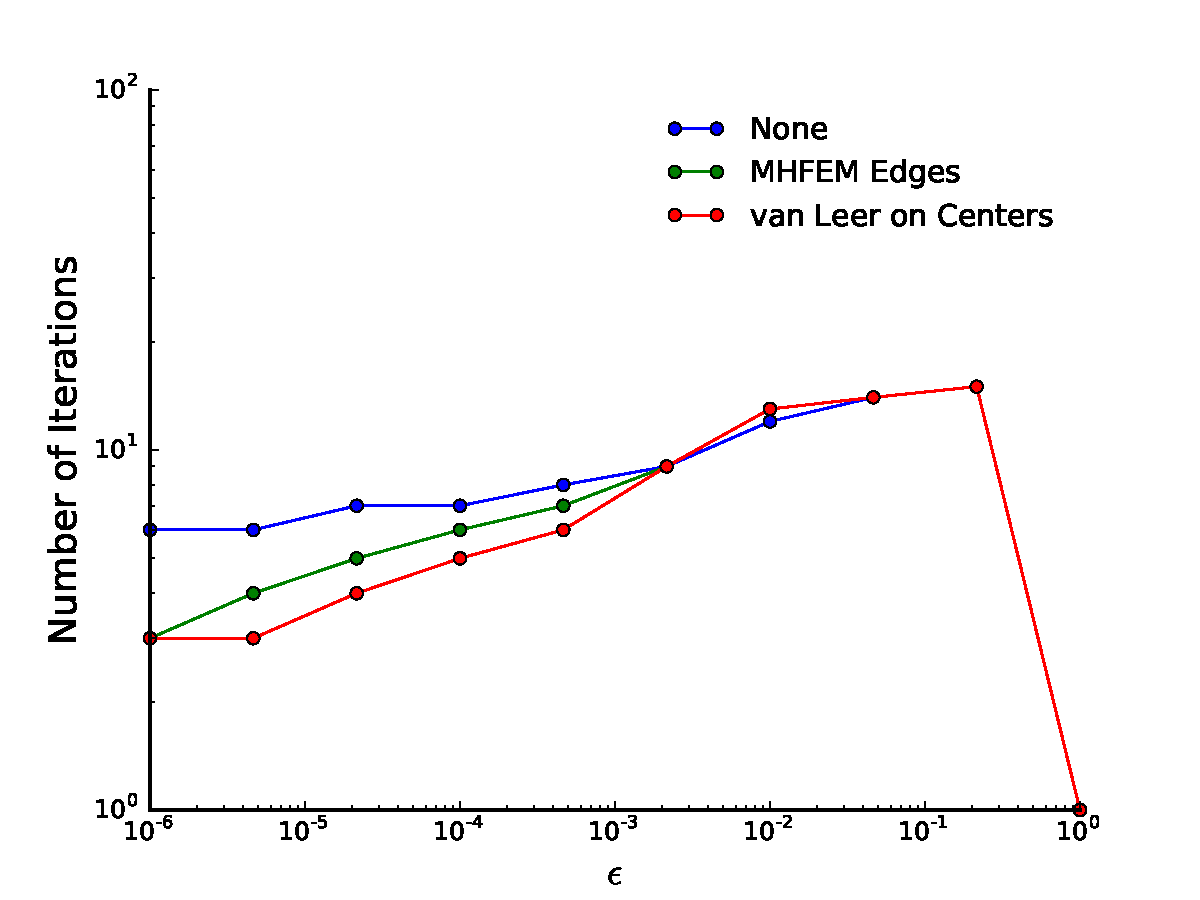
\includegraphics[width=.75\textwidth]{figs/diffLimit.pdf}
		\caption{The number of iterations for the VEF method to converge in the limit as $\epsilon \rightarrow 0$.}
		\label{fig:diffLim_iterations}
	\end{figure}
	\begin{figure} \centering
		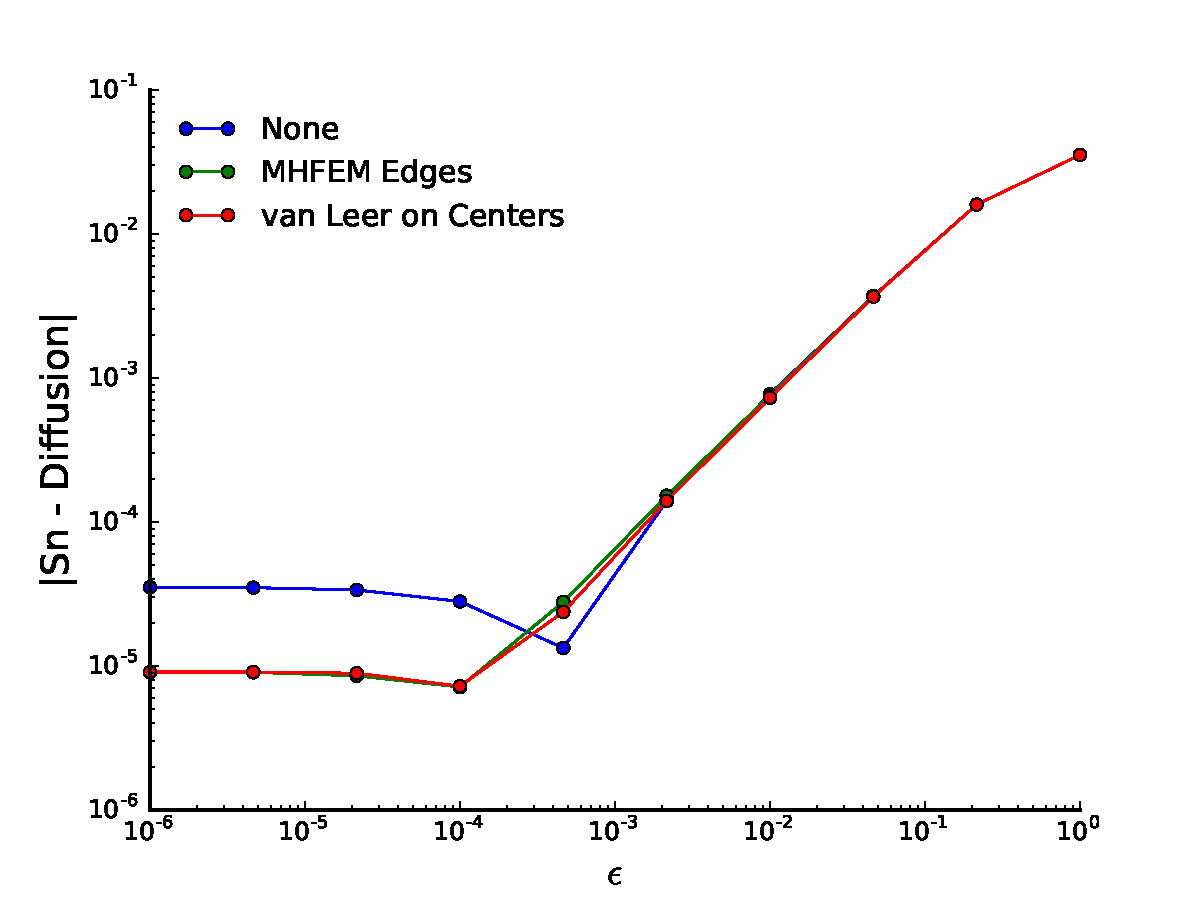
\includegraphics[width=.75\textwidth]{figs/diffError.pdf}
		\caption{A plot of the error between Diffusion Theory and the VEF solution as $\epsilon\rightarrow 0$. }
		\label{fig:diffLim_error}
	\end{figure}

\subsection{Solution Convergence}
The convergence between unaccelerated SI and the VEF method was compared as a function of cell width for a simple homogeneous slab and for a variant of Reed's problem. In both cases, the slab had a reflecting left boundary and vacuum right boundary. The homogeneous slab had a scattering ratio of 0.75. The cross sections and source for Reed's problem are provided in Table \ref{tab:reedXS}. Figure \ref{fig:reed} shows the L2 norm of the difference between unaccelerated and VEF accelerated S$_8$ for the two test problems. 

	\begin{table} \centering
		\begin{tabular}{|c|c|c|c|c|c|}
			\hline
			& Region 1 & Region 2 & Region 3 & Region 4 & Region 5 \\ 
			\hline 
			$q$ & 50 & 0 & 0 & 0 & 1 \\ 
			$\Sigma_t$ & 50 & 0.001 & 1 & 5 & 1 \\ 
			$\Sigma_a$ & 50 & 0 & 0.1 & 0 & 0.1 \\ 
			\hline 
			Domain & $0 \leq x < 2$ & $2 \leq x < 4$ & $4\leq x < 6$ &
				$6 \leq x < 7$ & $7 \leq x \leq 8$\\ 
			\hline 
		\end{tabular}
		\caption{The cross sections and source used for Reed's problem.}
		\label{tab:reedXS}
	\end{table}

	\begin{figure} \centering
		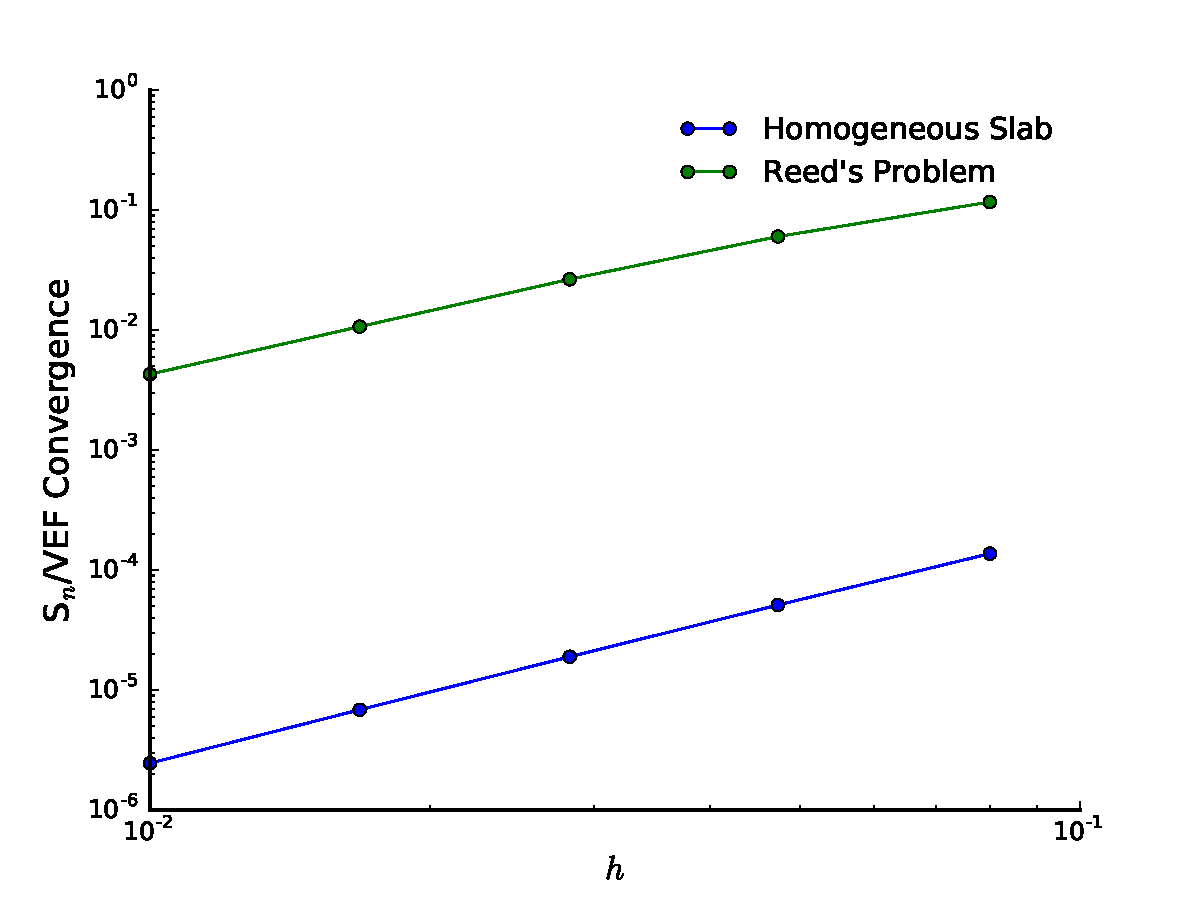
\includegraphics[width=.75\textwidth]{figs/convergence.pdf}
		\caption{The L2 norm of the difference between unaccelerated and VEF S$_8$ for a homogeneous slab and Reed's problem. }
		\label{fig:reed}
	\end{figure}

In both cases, the \SN and VEF solutions converge as the cell width is decreased. The convergence for Reed's problem is three orders of magnitudes worse than for the homogeneous slab case. This suggests that 

\subsection{Comparison to S$_2$SA}



\section{Conclusions and Future Work}


\begin{thebibliography}{99}
\bibitem{pomraning} Pomraning, G. C. (1964). A generalized P$_N$ approximation for neutron transport
problems. \emph{Nukleonik} 6:348.
\bibitem{ganguley} Ganguley, K., Allen, E. J., Coskun, E., and Nielsen, S. (1993). 
On the discrete-ordinates method via Case's solution, \emph{J. Comp. Phys.}, 107:66.
\bibitem{morel} Morel, J. E. (1989). A hybrid collocation-Galerkin-$S_N$  method for solving the
Boltzmann transport equation, {\emph Nucl. Sci. and Eng.}, 101:72.
\bibitem{DLMF}  Digital Library of Mathematical Functions.2011-08-29.National Institute of Standards and Technology from URL http://dlmf.nist.gov/14.7E11.
\bibitem{larsen1} Larsen, E. W., McGhee, J. M., Morel, J. E. (1992). The simplified P$_N$ equations
as an asymptotic limit of the transport equation. \emph{Trans. Am. Nucl. Soc.} 66:231.
\bibitem{larsen2} Larsen, E. W., Morel, J. E., McGhee, J. M. (1996). Asymptotic derivation of the
multigroup P$_1$ and simplified $P_N$ equations with anisotropic scattering. \emph{Nucl. Sci. Eng.}
123:328.
\bibitem{larsen3} Larsen, E. W., Asymptotic diffusion and simplified Pn
approximations for diffusive and deep
penetration problems. part 1: theory. (2011) \emph{TTSP} 39:110.
\end{thebibliography} 
\end{document}